%% (Master) Thesis template
% Template version used: v1.4
%
% Largely adapted from Adrian Nievergelt's template for the ADPS
% (lecture notes) project.


%% We use the memoir class because it offers a many easy to use features.
\documentclass[12pt,a4paper,titlepage]{memoir}

% no book layout now
\setulmarginsandblock{4cm}{4cm}{*}
\setlrmarginsandblock{4cm}{4cm}{*}

%% Packages
%% ========

%% LaTeX Font encoding -- DO NOT CHANGE
\usepackage[OT1]{fontenc}

%% Babel provides support for languages.  'english' uses British
%% English hyphenation and text snippets like "Figure" and
%% "Theorem". Use the option 'ngerman' if your document is in German.
%% Use 'american' for American English.  Note that if you change this,
%% the next LaTeX run may show spurious errors.  Simply run it again.
%% If they persist, remove the .aux file and try again.
\usepackage[ngerman]{babel}

%% Input encoding 'utf8'. In some cases you might need 'utf8x' for
%% extra symbols. Not all editors, especially on Windows, are UTF-8
%% capable, so you may want to use 'latin1' instead.
\usepackage[utf8]{inputenc}

%% This changes default fonts for both text and math mode to use Herman Zapfs
%% excellent Palatino font.  Do not change this.
\usepackage[sc]{mathpazo}

%% The AMS-LaTeX extensions for mathematical typesetting.  Do not
%% remove.
\usepackage{amsmath,amssymb,amsfonts,mathrsfs}

%% NTheorem is a reimplementation of the AMS Theorem package. This
%% will allow us to typeset theorems like examples, proofs and
%% similar.  Do not remove.
%% NOTE: Must be loaded AFTER amsmath, or the \qed placement will
%% break
\usepackage[amsmath,thmmarks]{ntheorem}

%% LaTeX' own graphics handling
\usepackage{graphicx}

\graphicspath{ {bilder/} }

%% We unfortunately need this for the Rules chapter.  Remove it
%% afterwards; or at least NEVER use its underlining features.
\usepackage{soul}

%% This allows you to add .pdf files. It is used to add the
%% declaration of originality.
\usepackage{pdfpages}

%% Some more packages that you may want to use.  Have a look at the
%% file, and consult the package docs for each.
%% See the TeXed file for more explanations

%% [OPT] Multi-rowed cells in tabulars
%\usepackage{multirow}

%% [REC] Intelligent cross reference package. This allows for nice
%% combined references that include the reference and a hint to where
%% to look for it.
\usepackage{varioref}

%% [OPT] Easily changeable quotes with \enquote{Text}
%\usepackage[german=swiss]{csquotes}

%% [REC] Format dates and time depending on locale
\usepackage{datetime}

%% [OPT] Provides a \cancel{} command to stroke through mathematics.
%\usepackage{cancel}

%% [NEED] This allows for additional typesetting tools in mathmode.
%% See its excellent documentation.
\usepackage{mathtools}

%% [ADV] Conditional commands
%\usepackage{ifthen}

%% [OPT] Manual large braces or other delimiters.
%\usepackage{bigdelim, bigstrut}

%% [REC] Alternate vector arrows. Use the command \vv{} to get scaled
%% vector arrows.
\usepackage[h]{esvect}

%% [NEED] Some extensions to tabulars and array environments.
\usepackage{array}

%% [OPT] Postscript support via pstricks graphics package. Very
%% diverse applications.
%\usepackage{pstricks,pst-all}

%% [?] This seems to allow us to define some additional counters.
%\usepackage{etex}

%% [ADV] XY-Pic to typeset some matrix-style graphics
%\usepackage[all]{xy}

%% [OPT] This is needed to generate an index at the end of the
%% document.
%\usepackage{makeidx}

%% [OPT] Fancy package for source code listings.  The template text
%% needs it for some LaTeX snippets; remove/adapt the \lstset when you
%% remove the template content.
\usepackage{listings}
\lstset{language=TeX,basicstyle={\normalfont\ttfamily}}
%% [REC] Fancy character protrusion.  Must be loaded after all fonts.
\usepackage[activate]{pdfcprot}

%% [REC] Nicer tables.  Read the excellent documentation.
\usepackage{booktabs}


%% Our layout configuration.  DO NOT CHANGE.
%% Memoir layout setup

%% NOTE: You are strongly advised not to change any of them unless you
%% know what you are doing.  These settings strongly interact in the
%% final look of the document.

% Dependencies
\usepackage{HSLUlogo}

% Turn extra space before chapter headings off.
\setlength{\beforechapskip}{0pt}

\nonzeroparskip
\parindent=0pt
\defaultlists

% Chapter style redefinition
\makeatletter

\if@twoside
  \pagestyle{Ruled}
  \copypagestyle{chapter}{Ruled}
\else
  \pagestyle{ruled}
  \copypagestyle{chapter}{ruled}
\fi
\makeoddhead{chapter}{}{}{}
\makeevenhead{chapter}{}{}{}
\makeheadrule{chapter}{\textwidth}{0pt}
\copypagestyle{abstract}{empty}

\makechapterstyle{bianchimod}{%
  \chapterstyle{default}
  \renewcommand*{\chapnamefont}{\normalfont\Large\sffamily}
  \renewcommand*{\chapnumfont}{\normalfont\Large\sffamily}
  \renewcommand*{\printchaptername}{%
    \chapnamefont\centering\@chapapp}
  \renewcommand*{\printchapternum}{\chapnumfont {\thechapter}}
  \renewcommand*{\chaptitlefont}{\normalfont\huge\sffamily}
  \renewcommand*{\printchaptertitle}[1]{%
    \hrule\vskip\onelineskip \centering \chaptitlefont\textbf{\vphantom{gyM}##1}\par}
  \renewcommand*{\afterchaptertitle}{\vskip\onelineskip \hrule\vskip
    \afterchapskip}
  \renewcommand*{\printchapternonum}{%
    \vphantom{\chapnumfont {9}}\afterchapternum}}

% Use the newly defined style
\chapterstyle{bianchimod}

\setsecheadstyle{\Large\bfseries\sffamily}
\setsubsecheadstyle{\large\bfseries\sffamily}
\setsubsubsecheadstyle{\bfseries\sffamily}
\setparaheadstyle{\normalsize\bfseries\sffamily}
\setsubparaheadstyle{\normalsize\itshape\sffamily}
\setsubparaindent{0pt}

% Set captions to a more separated style for clearness
\captionnamefont{\sffamily\bfseries\footnotesize}
\captiontitlefont{\sffamily\footnotesize}
\setlength{\intextsep}{16pt}
\setlength{\belowcaptionskip}{1pt}

% Set section and TOC numbering depth to subsection
\setsecnumdepth{subsection}
\settocdepth{subsection}

%% Titlepage adjustments
\pretitle{\vspace{0pt plus 0.7fill}\begin{center}\HUGE\sffamily\bfseries}
\posttitle{\end{center}\par}
\preauthor{\par\begin{center}\let\and\\\Large\sffamily}
\postauthor{\end{center}}
\predate{\par\begin{center}\Large\sffamily}
\postdate{\end{center}}

\def\@advisors{}
\newcommand{\advisors}[1]{\def\@advisors{#1}}
\def\@department{}
\newcommand{\department}[1]{\def\@department{#1}}
\def\@thesistype{}
\newcommand{\thesistype}[1]{\def\@thesistype{#1}}

\renewcommand{\maketitlehooka}{\noindent\HSLUlogo[2in]}

\renewcommand{\maketitlehookb}{\vspace{1in}%
  \par\begin{center}\Large\sffamily\@thesistype\end{center}}

\renewcommand{\maketitlehookd}{%
  \vfill\par
  \begin{flushright}
    \sffamily
    \@advisors\par
    \@department, Hochschule Luzern
  \end{flushright}
}

\checkandfixthelayout

\setlength{\droptitle}{-48pt}

\makeatother

% This defines how theorems should look. Best leave as is.
\theoremstyle{plain}
\setlength\theorempostskipamount{0pt}

%%% Local Variables:
%%% mode: latex
%%% TeX-master: "thesis"
%%% End:


%% Theorem environments.  You will have to adapt this for a German
%% thesis.
%% Theorem-like environments

%% This can be changed according to language. You can comment out the ones you
%% don't need.

\numberwithin{equation}{chapter}

%% German theorems
%\newtheorem{satz}{Satz}[chapter]
%\newtheorem{beispiel}[satz]{Beispiel}
%\newtheorem{bemerkung}[satz]{Bemerkung}
%\newtheorem{korrolar}[satz]{Korrolar}
%\newtheorem{definition}[satz]{Definition}
%\newtheorem{lemma}[satz]{Lemma}
%\newtheorem{proposition}[satz]{Proposition}

%% English variants
\newtheorem{theorem}{Theorem}[chapter]
\newtheorem{example}[theorem]{Example}
\newtheorem{remark}[theorem]{Remark}
\newtheorem{corollary}[theorem]{Corollary}
\newtheorem{definition}[theorem]{Definition}
\newtheorem{lemma}[theorem]{Lemma}
\newtheorem{proposition}[theorem]{Proposition}

%% Proof environment with a small square as a "qed" symbol
\theoremstyle{nonumberplain}
\theorembodyfont{\normalfont}
\theoremsymbol{\ensuremath{\square}}
\newtheorem{proof}{Proof}
%\newtheorem{beweis}{Beweis}


%% Helpful macros.
%% Custom commands
%% ===============

%% Special characters for number sets, e.g. real or complex numbers.
\newcommand{\C}{\mathbb{C}}
\newcommand{\K}{\mathbb{K}}
\newcommand{\N}{\mathbb{N}}
\newcommand{\Q}{\mathbb{Q}}
\newcommand{\R}{\mathbb{R}}
\newcommand{\Z}{\mathbb{Z}}
\newcommand{\X}{\mathbb{X}}

%% Fixed/scaling delimiter examples (see mathtools documentation)
\DeclarePairedDelimiter\abs{\lvert}{\rvert}
\DeclarePairedDelimiter\norm{\lVert}{\rVert}

%% Use the alternative epsilon per default and define the old one as \oldepsilon
\let\oldepsilon\epsilon
\renewcommand{\epsilon}{\ensuremath\varepsilon}

%% Also set the alternate phi as default.
\let\oldphi\phi
\renewcommand{\phi}{\ensuremath{\varphi}}


%% Make document internal hyperlinks wherever possible. (TOC, references)
%% This MUST be loaded after varioref, which is loaded in 'extrapackages'
%% above.  We just load it last to be safe.
\usepackage[linkcolor=black,colorlinks=true,citecolor=black,filecolor=black]{hyperref}


%% longtable
\usepackage{longtable}

%% Document information
%% ====================

\title{Prototyping einer webbasierten Visualisierung zur intuitiven Interaktion mit einem Wissensnetzwerk}
\author{Andreas Waldis, Patrick Siegfried}
\thesistype{}
\advisors{Advisor: Dr.\ Michael Kaufmann}
\department{Departement Informatik}
\date{\today}

\begin{document}

\frontmatter

%% Title page is autogenerated from document information above.  DO
%% NOT CHANGE.
\begin{titlingpage}
  \calccentering{\unitlength}
  \begin{adjustwidth*}{\unitlength-24pt}{-\unitlength-24pt}
    \maketitle
  \end{adjustwidth*}
\end{titlingpage}

%% The abstract of your thesis.  Edit the file as needed.
\begin{abstract}
  Im Rahmen des Informatikprojekts wurde ein Prototyp für die Visualisierung und Interaktion von \gls{Netzwerk}[en] erarbeitet. Dazu wurden mithilfe der Spezifikation von funktionalen Anforderungen verschiedene \gls{Framework}[s] für die Grundlage der Entwicklung evaluiert. Anschliessend wurde die für den Anwendungsfall beste Wahl getroffen.
  
  Der Prototyp bietet eine Benutzeroberfläche, welche sowohl auf kleinen und grossen Bildschirmen, mit Touch-Gesten oder der Maus und der Tastatur, verwendet werden kann.
  Der resultierende Prototyp wurde als selbständiges Software-Paket entwickelt. Dadurch kann dieser in beliebigen Applikationen verwendet werden. In der letzten Projektphase wurde der Prototyp schlussendlich in den bestehenden \gls{ikc-core} integriert.
\end{abstract}


%% TOC with the proper setup, do not change.
\cleartorecto
\tableofcontents
\mainmatter

%% Your real content!
\chapter{Einleitung}

Im Hasler-Projekt Intuitive Knowledge Connectivity (IKC) wird ein Prototyp für plattformübergreifendes Wissensnetzwerk erstellt. Die grundlegende Datenbank basiert auf einen Netzwerk (einem gerichteten beschrifteten Property-Graph), hat aber bisher nur eine technische Konsole. Eine ideale grafische Benutzerschnittstelle stellt das Netzwerk oder Teilausschnitte daraus visuell und zweidimensional dar, und stellt beschriftete Knoten und Pfeile grafisch dar. Dies ermöglicht eine einfache und übersichtliche Repräsentation und eine intuitive Interaktion mit den gegebenen Kanten und Knoten. Der bestehende Prototyp implementiert die grundlegenden Datenbankoperationen (CRUD) und die Verknüpfung von Knoten mit Drag and Drop. Auf dieser Kern-Software soll aufgebaut werden, um diese hinsichtlich intuitiver Benutzung zu erweitern, damit mit mehreren Knoten im Netzwerk gleichzeitig und visuell gearbeitet werden kann. Dies soll in erster Linie auf dem Touchscreen (mobil / Tablet) und in zweiter Linie responsive mit dem gleichen Code auch mit Bildschirm, Tastatur und Maus / Touchpad bedienbar sein.

\chapter{Lösungskonzept}

Das Lösungskonzept beinhaltet die Grundlagen für die erfolgreiche Umsetzung des Prototypen. Der Inhalt ist hauptsächlich aus den Bereich Management und Anforderungen. Die unter Anforderungen aufgenommenen Punkte sind in Zusammenarbeit mit dem Projektpartner entstanden, um so auch die Ansprüche des Forschungsprojektes zu erfüllen.

\section{Projektmanagement}

Führung und Kontrolle des Projekte werden im folgenden Kapitel aufgezeigt. Das Management funktioniert agil, dafür werden geeignete Methoden (vgl. \textit{ScrumDo}) eingesetzt.

\subsection{Projektstrukturplan}
Die \autoref{fig:projektstrukturplan} gewährt einen Überblick über das Projekt. Sie stellt die wichtigsten Bereich und Phasen dar, worin die Arbeit grob eingegliedert werden kann.

\begin{figure}[ht]
\centering
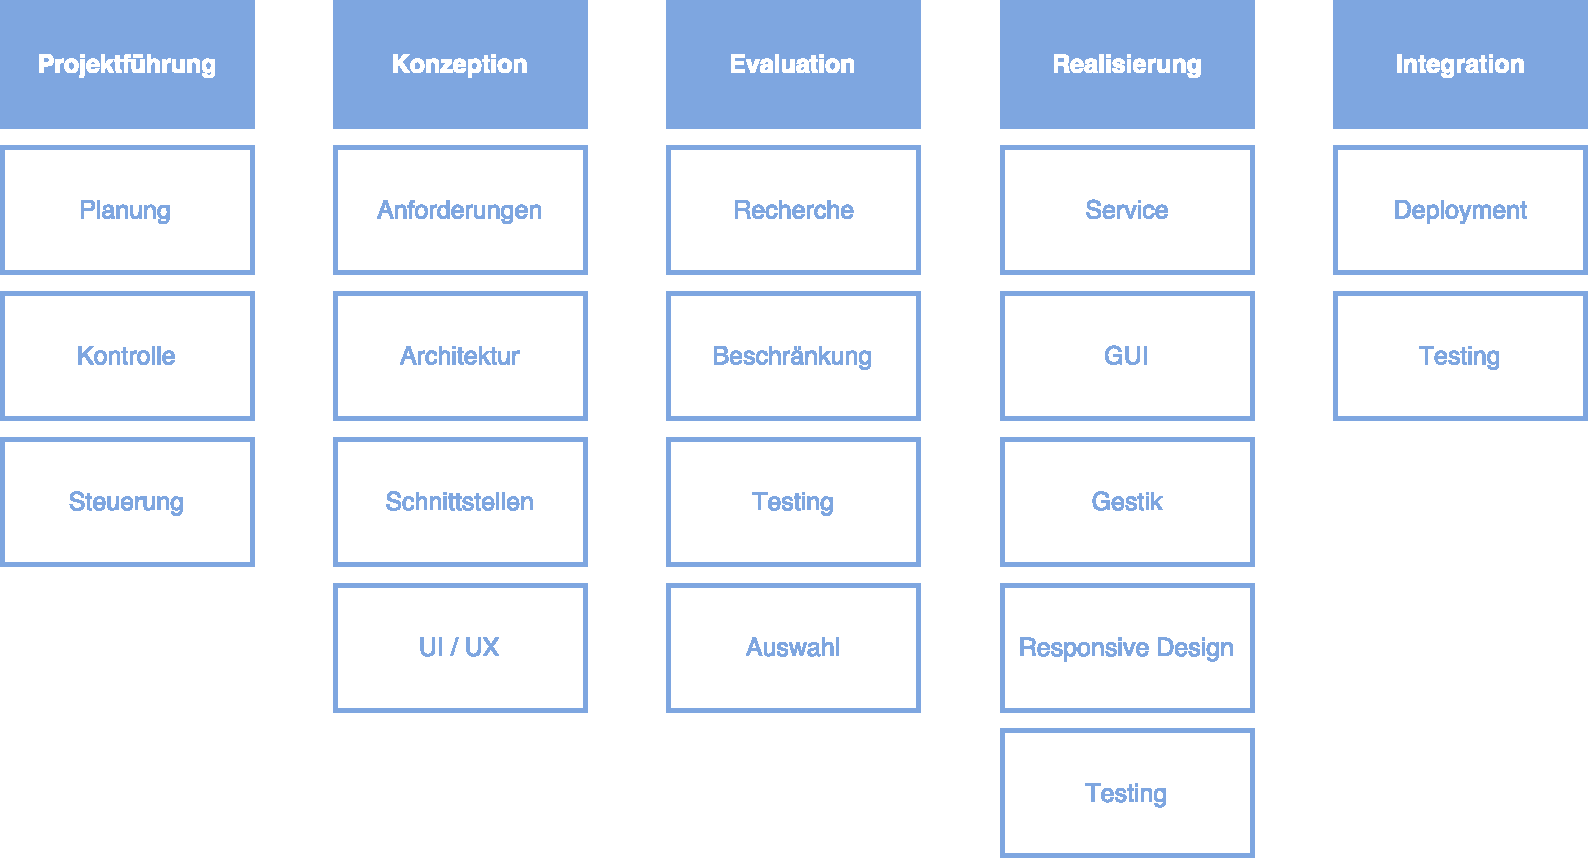
\includegraphics[width=0.7\textwidth]{Projektstrukturplan}
\caption{Projektstrukturplan}
\label{fig:projektstrukturplan}
\end{figure}


\subsection{Projektführung}



\section{Anforderungen}

Für die weitere Unterteilung in Arbeitspakete und Stories, werden die Anforderungen zunächst in Prosa gesammelt. Diese entstammen dem Kundenworkshop und der Aufgabenstellung.

\subsection{Projektmanagement}

\begin{enumerate}
    \item Das Projekt wird agil in allen Bereichen agil geführt.
\end{enumerate}

\subsection{Funktionale Anforderungen}

\begin{table}
  \centering
  \begin{tabular}{|p{0.6cm} | p{1.6cm} | p{8cm}|}
  \hline
    ID & Priorität & Beschreibung \\\hline
    A1 & X & Die zugrunde liegende Datenbasis kann mittels eines Graphen visualisiert werden. Jener besteht aus Knoten und Kanten, welche gerichtet und beschriftet sind.\\\hline
    A2 & X & Der zu erarbeitende Prototyp kann bidirektional mit dem \textit{ikc-core}-Prototypen interagieren. Änderungen am \textit{ikc-core} sind in der Visualisierung sichtbar. Es ist jedoch es auch möglich Änderungen direkt in der Visualisierung vorzunehmen.\\\hline
    A3 & X & Mittels der Visualisierung können die grundlegenden Datenbankoperationen \textit{CREATE}, \textit{READ}, \textit{UPDATE} und \textit{DELETE} (CRUD) direkt auf der Datenbasis des \textit{ikc-core} angewendet werden.\\\hline
    A4 & X & Der Prototyp kann auf Smartphones und Tablets benutzt werden.\\\hline
    A5 & X & Der Prototyp kann auf Laptops und Desktop-Computern benutzt werden.\\\hline    
    A6 & X & Mit Hilfe verschiedener Kriterien (beispielsweise Kontext oder Nachbarschaft) kann ein Teilgraph visualisiert werden.\\\hline 
    A7 & X & Die Visualisierung kann in verschiedenen Projekten wiederverwendet werden.\\\hline     
     
  \end{tabular}
    \caption{Funktionale Anforderungen}
  \label{tab:funktionale-anforderungen}
\end{table}

\begin{enumerate}
    \item Die zugrunde liegende Datenbasis kann mittels eines Graphen visualisiert werden. Jener besteht aus Knoten und Kanten, welche gerichtet und beschriftet sind.
    \item Der zu erarbeitende Prototyp kann bidirektional mit dem \textit{ikc-core}-Prototypen interagieren. Änderungen am \textit{ikc-core} sind in der Visualisierung sichtbar. Es ist jedoch es auch möglich Änderungen direkt in der Visualisierung vorzunehmen.
    \item Mittels der Visualisierung können die grundlegenden Datenbankoperationen \textit{CREATE}, \textit{READ}, \textit{UPDATE} und \textit{DELETE} (CRUD) direkt auf der Datenbasis des \textit{ikc-core} angewendet werden.
    \item Die Entwicklung erfolgt nach dem Ansatz \textit{mobile-first}, was bedeutet, dass absteigend nach der Priorität die Darstellung für die folgenden Plattformen, Mobile, Tablet, Laptop und Desktop, entwickelt wird.
    \item Der Prototyp kann auf Smartphones und Tablets benutzt werden.
    \item Der Prototyp kann auf Laptops und Desktop-Computern benutzt werden.
    \item Mit Hilfe verschiedener Kriterien (beispielsweise Kontext oder Nachbarschaft) kann ein Teilgraph visualisiert werden.
    \item Die Visualisierung kann in verschiedenen Projekten wiederverwendet werden.
\end{enumerate}

\subsection{Nicht funktionale Anforderungen}

\begin{table}
  \centering
  \begin{tabular}{|p{0.4cm} | p{1.3cm} | p{8cm}|}
  \hline
     ID & Priorität & Beschreibung \\\hline
     1 & X & Die zugrunde liegende Datenbasis kann mittels eines Graphen visualisiert werden. Jener besteht aus Knoten und Kanten, welche gerichtet und beschriftet sind.\\\hline
     2 & X & Die zugrunde liegende Datenbasis kann mittels eines Graphen visualisiert werden. Jener besteht aus Knoten und Kanten, welche gerichtet und beschriftet sind.\\\hline
     
  \end{tabular}
    \caption{Nicht funktionale Anforderungen}
  \label{tab:nicht-funktionale-anforderungen}
\end{table}

\begin{enumerate}
    \item Die Visualisierung kann direkt nahtlos innerhalb des \textit{ikc-core} verwendet werden.
    \item Bestehende Funktionen (beispielsweise \textit{New Node}, \ldots) können teilweise direkt in der Visualisierung dargestellt werden.
    \item Der zu entwicklende Prototyp kann zur Verfügung stehende Schnittstellen des \textit{ikc-core} verwenden.
    \item Der Prototyp kann (unter anderem) mit Drag and Drop bedient werden.
\end{enumerate}


\section{Stories}

\begin{table}
  \centering
  \caption{Things you (usually) don't say}
  \label{tab:things-you-dont-say}
  \begin{tabular}{lll}
    \toprule
    \st{It holds (that) \dots} & We have \dots & \emph{Es gilt \dots}\\
    \multicolumn{3}{l}{\quad\footnotesize(`Equation (5) holds.' is fine, though.)}\\
    \st{$x$ fulfills property $\mathcal{P}$.}& \(x\) satisfies property \(\mathcal{P}\). & \emph{\(x\) erfüllt Eigenschaft \(\mathcal{P}\).} \\
    \st{in average} & on average & \emph{im Durchschnitt}\\
    \st{estimation} & estimate   & \emph{Abschätzung}\\
    \st{composed number} & composite number & \emph{zusammengesetzte Zahl}\\
    \st{with the help of} & using & \emph{mit Hilfe von}\\
    \st{surely} & clearly & \emph{sicher, bestimmt}\\
    \st{monotonously increasing} & monotonically incr. & \emph{monoton steigend}\\
    \multicolumn{3}{l}{\quad\footnotesize(Actually, in most cases `increasing' is just fine.)}\\
    \bottomrule
  \end{tabular}
\end{table}


\chapter{Implementation}

\chapter{Schlussfolgerungen}

\chapter{Literatur}

\chapter{Anhang}

\appendix

\chapter{Dummy Appendix}

You can defer lengthy calculations that would otherwise only interrupt
the flow of your thesis to an appendix.


\backmatter

\bibliographystyle{plain}
\bibliography{refs}

%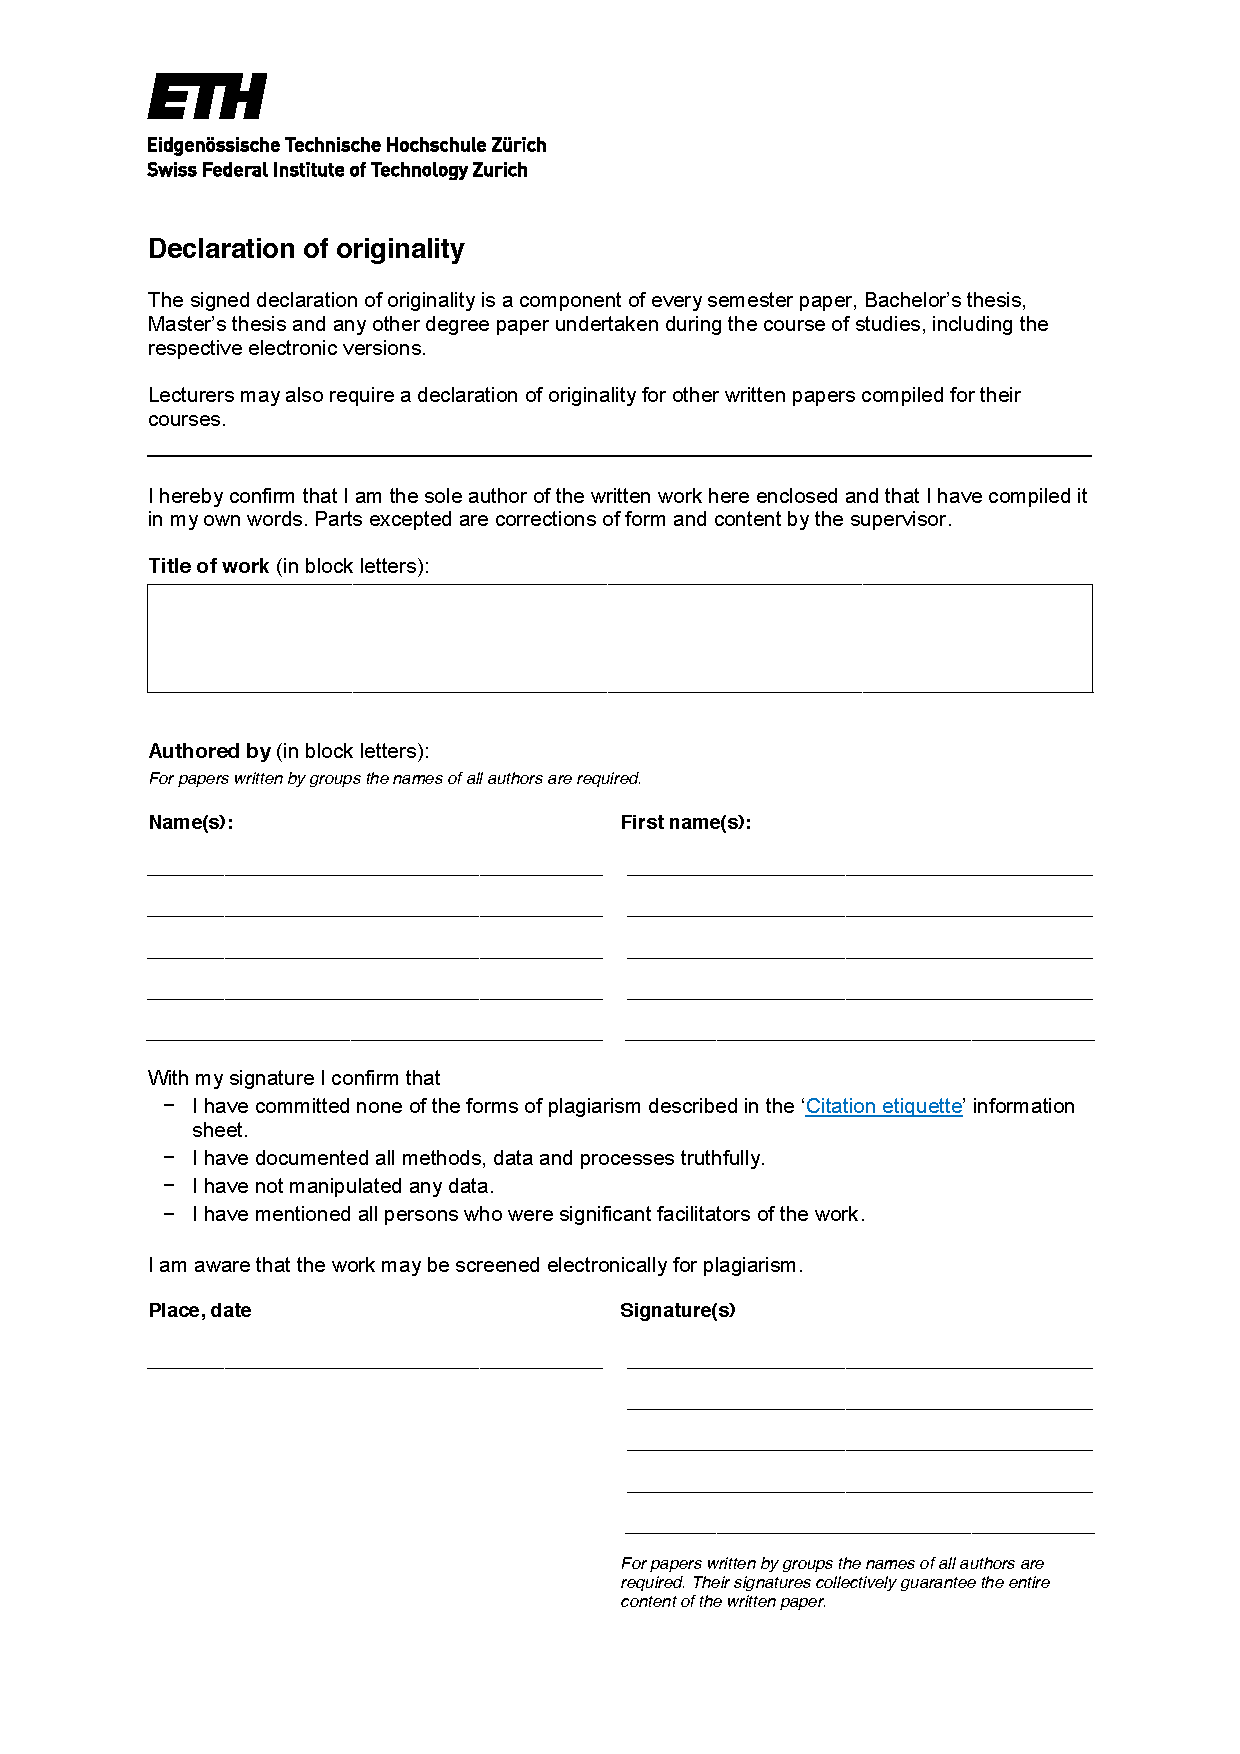
\includepdf[pages={-}]{declaration-originality.pdf}

\end{document}
